\chapter{Infectious disease mechanism}

Viruses are universally dependent upon their host cell. Despite the diverse functions that viruses encode for their propagation, they remain exquisitely dependent on the translational machinery of the host cell. No matter whether their genomes are RNA or DNA, and regardless of their mRNA production method, the goal remains the same: to ensure that cellular ribosomes are recruited to viral mRNAs \cite{Walsh:2011kt}.

\begin{figure*}
\center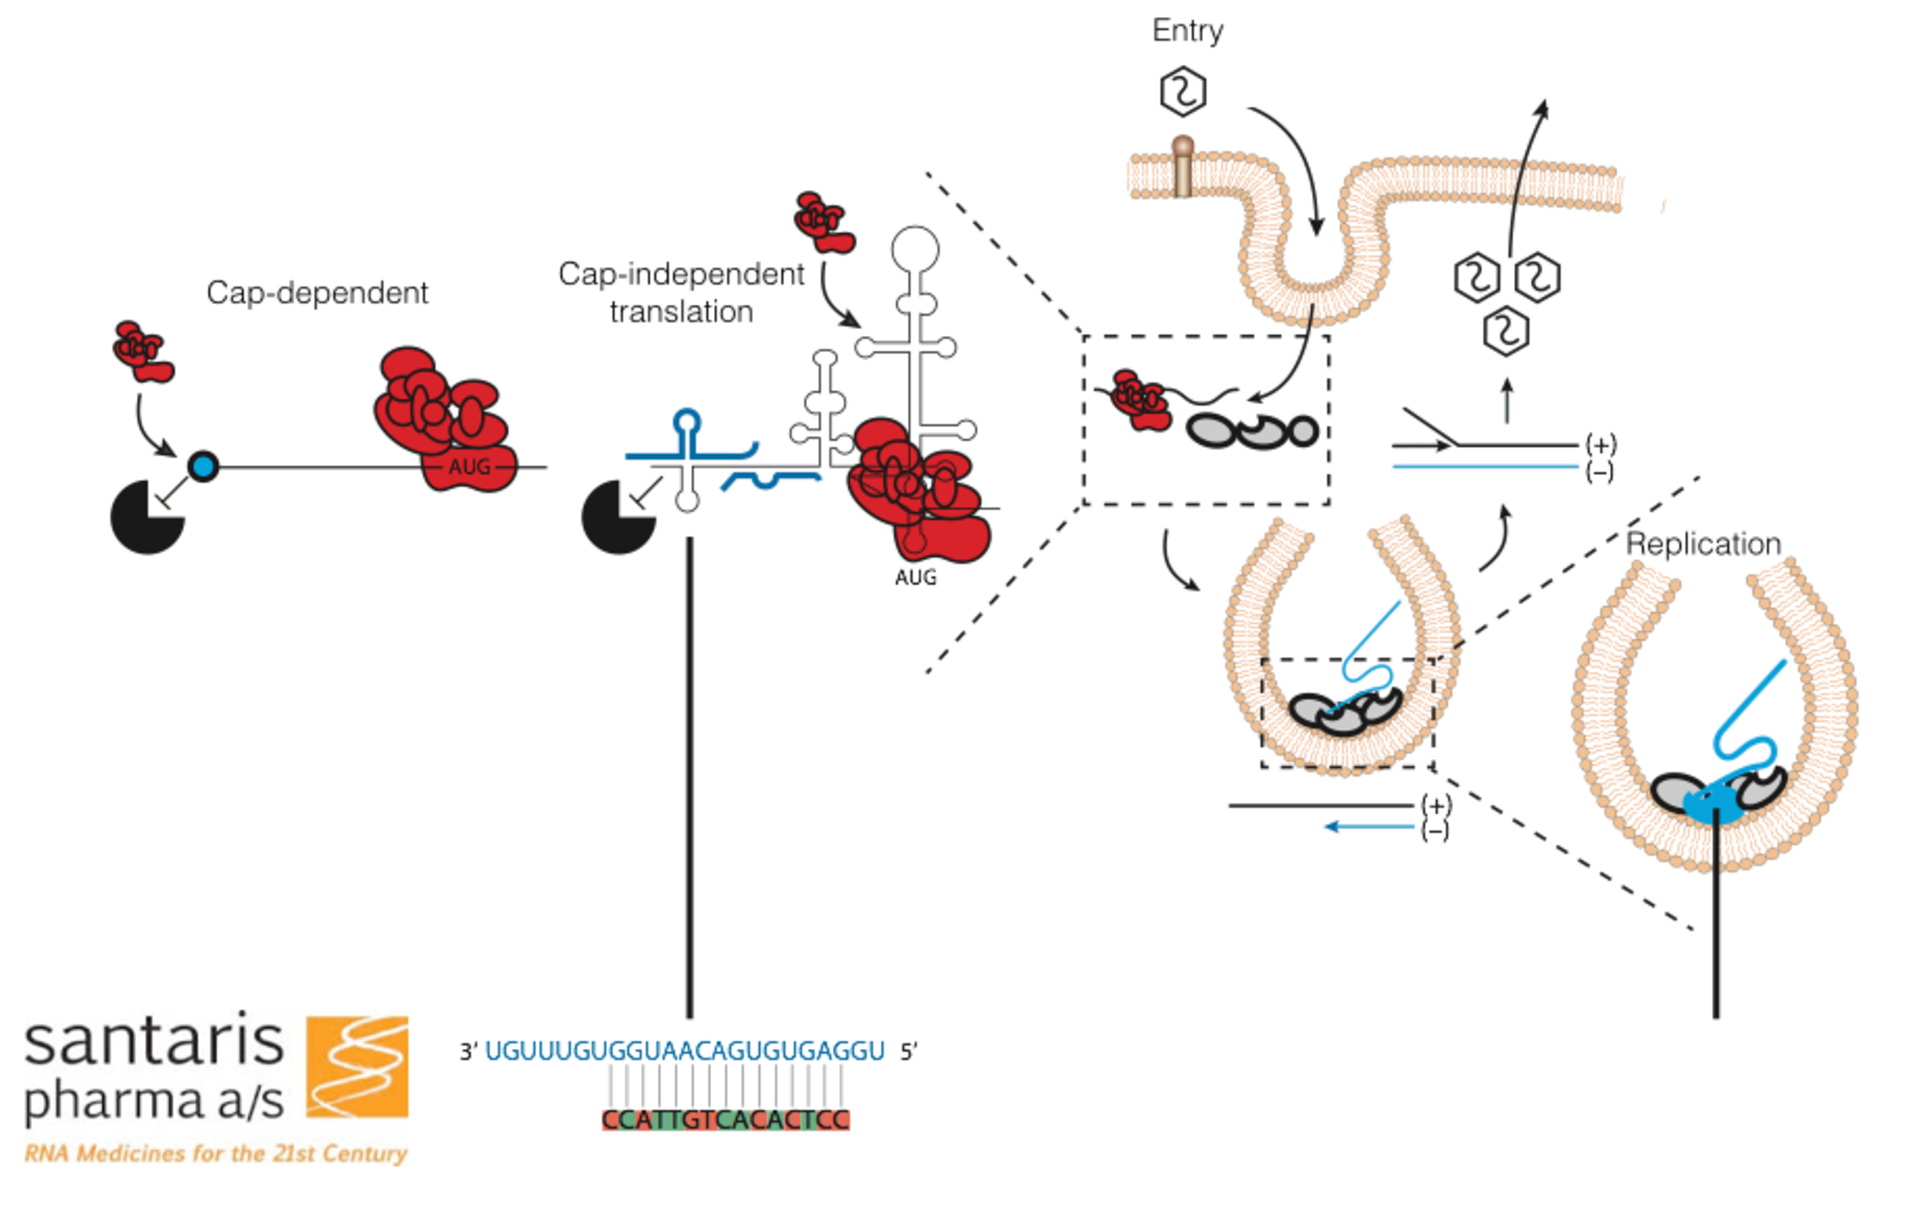
\includegraphics[width=140mm,scale=0.5]{Figures/Fig19}
\caption{Different modes of translation.}
\label{fig:Fig19}
\end{figure*}

Cellular mRNAs use cap-dependent translation, a process that involves interaction between initiation-factor proteins and the 7-methyl guanosine cap at the 5$'$ end of mRNA. This leads to 40S ribosome binding and scanning to the initiation codon, which is then followed by association with the 60S ribosomal subunit to form an active 80S ribosome that initiates translation of the protein (Figure ~\ref{fig:Fig19}).

An alternative pathway, called internal translation initiation, is a cap-independent mechanism of recruiting, positioning, and activating the eukaryotic protein-synthesis machinery driven by structured RNA sequences called internal ribosome entry sites (IRESs) that are located in the 5$'$ -untranslated region (UTR) of certain mRNAs \cite{Fraser:2006kn}. Lacking a 5$'$ cap, many RNA viruses contain IRES that mediate cap-independent translation. In this process, the virus commandeers cellular ribosomes as well as translation factors and signalling pathways that control the host protein synthesis. 

\section{HCV}

IRES-mediated translation is well-studied in the context of HCV and the structure of the 5$'$ UTR region is well-understood \cite{Fraser:2006kn}. Because of this, HCV is an excellent model system for extending the CLIP pipeline into infectious diseases. We approached this study by first identifying a protein that was (1) known to bind the HCV genome and (2) was critical for HCV replication, but (3) for which the mechanism of action remained unclear. We chose Poly-C binding protein 2 (PCBP2), a well-characterized RNA-binding protein with several studies linking it to HCV \cite{GarciaSastre:2013ko}.

\begin{figure*}
\center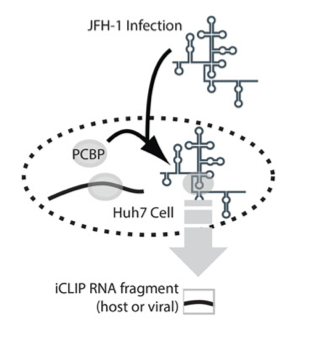
\includegraphics[width=80mm,scale=0.5]{Figures/Fig20}
\caption{CLIP applied to HCV virus.}
\label{fig:Fig20}
\end{figure*}

Though PCBP2 is required for HCV replication, the molecular details are poorly understood. Several studies focused on the HCV 5$'$ UTR have led to the suggestion that a complex between PCBP2 and SL1 of the 5$'$ UTR as well as an undefined region of the 3$'$ UTR of the viral RNA may be formed that facilitates viral circularization. Both SL1 and stem loop structures in the  3$'$ UTR of the viral genome are required for viral RNA replication. In addition, the proximity of SL1 to the conserved miR-122 sites in the HCV genome suggests that PCBP2 may coordinate with miR-122 in protection of the uncapped 5$'$ end of the viral RNA from degradation and/or the switch between viral translation and RNA replication \cite{GarciaSastre:2013ko}.


To elucidate the connection between PCBP2, translational regulation, and disease, we performed iCLIP in Huh-7 cells infected with the JFH-1 strain of Hepatitis C virus (HCV). We designed the pipeline so that it could easily be applied to viruses, and supplied the sequence of the JFH-1 genome as the mapping index (Figure ~\ref{fig:Fig20}). We generated coverage histograms of iCLIP RT stops across the HCV genome for two biological replicates, observing favorable concordance and global preference for binding U/C-rich regions of the genome ($r^2 = 0.93$) \cite{Flynn:2014bi}.

Consistent with prior studies, we observed a strong binding peak at SL1, but also detected PCBP2 occupancy that extends from SLI through the two miR-122 binding sites to the base of SL2. Surprisingly, we also detected strong binding around the translation start codon within SLVI of the internal ribosome entry site (IRES) (Figure ~\ref{fig:Fig21}). PCBP2$'$s interaction with viral 3$'$ UTR was significantly stronger than with the well-studied 5$'$ UTR. PCBP2 binding to the 3$'$ UTR occurred primarily in the single-stranded regions between stem-loops 5BSL3.2 and the variable region, a domain that includes the viral stop codon and that is implicated in both stimulation of translation and replication. Not surprisingly, PCBP2 also bound to the poly(U)/UC region of the viral genome, consistent with binding to single-stranded poly(U)/C regions. In addition to the UTRs, we observe multiple robust peaks of PCBP2 occupancy across the full viral gene body, which has never been reported.

\begin{figure*}
\center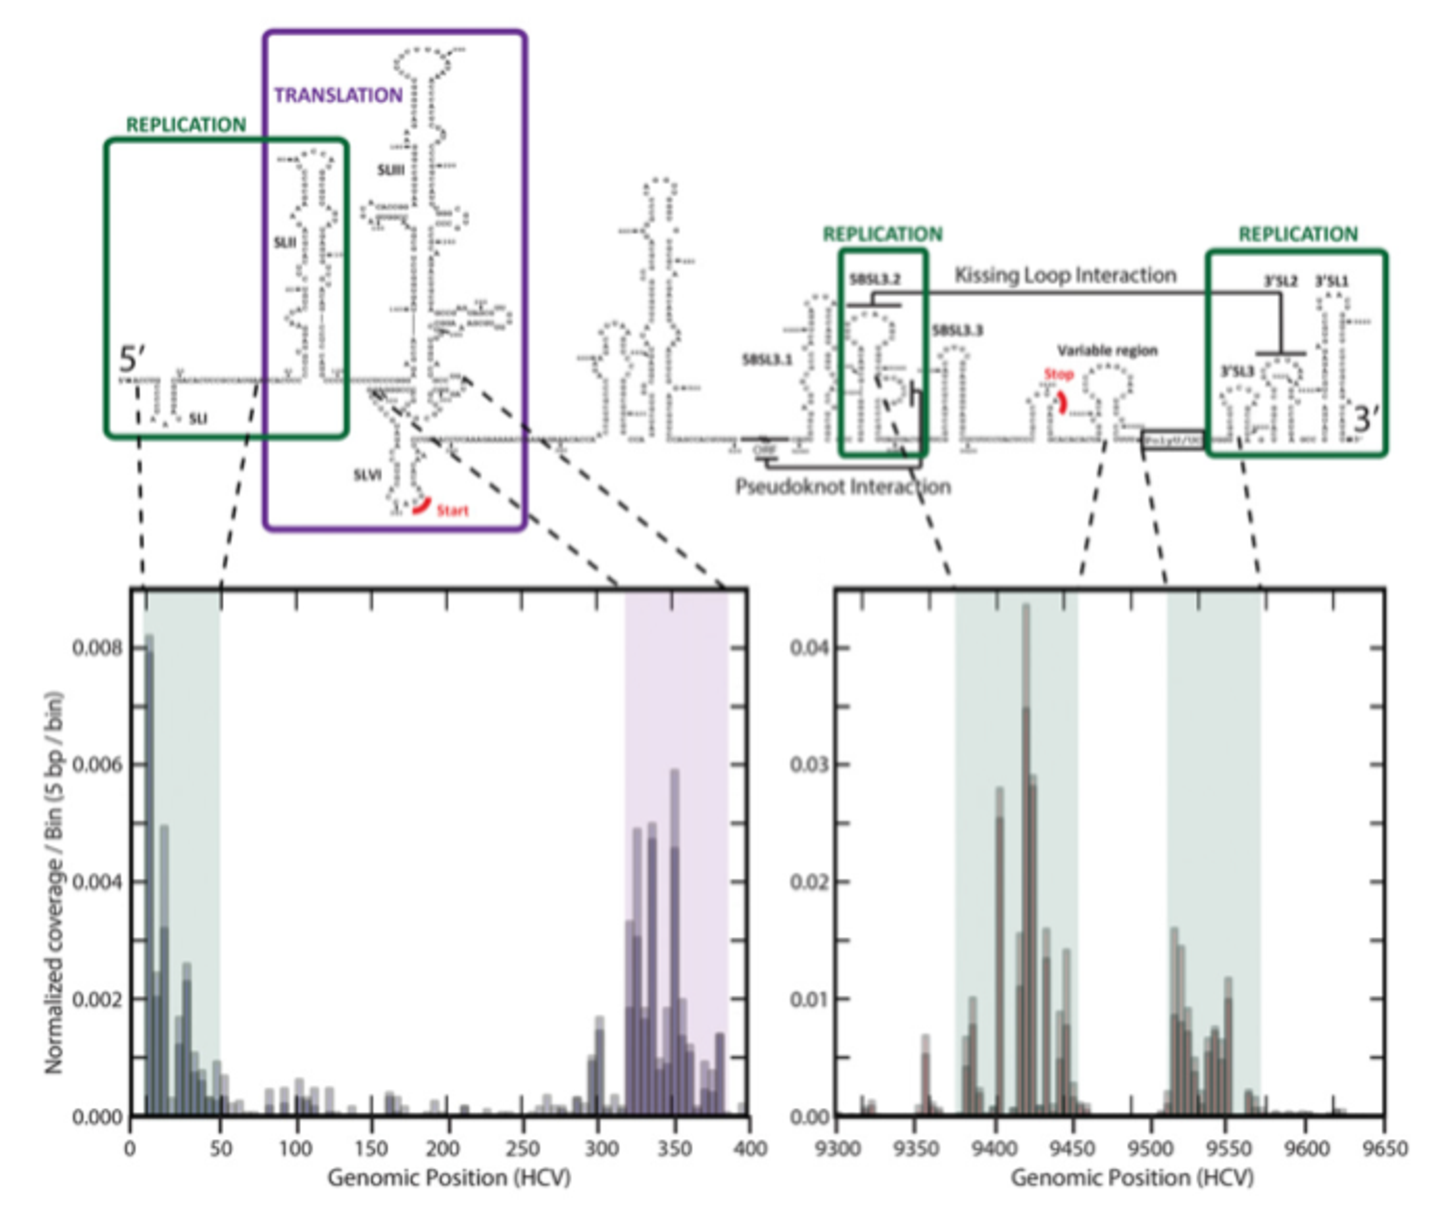
\includegraphics[width=150mm,scale=0.5]{Figures/Fig21}
\caption{PCBP binding profile on the HCV genome.}
\label{fig:Fig21}
\end{figure*}

Our application of FAST-iCLIP to HCV suggests that these regulatory functions of PCBP may be co-opted by the virus, as we also observe PCBP2 binding to the viral 5$'$ UTR, coding region, and 3$'$ UTR. We observe a peak of PCBP2 around the SL1/miR-122 binding site junction in the HCV genome, suggesting that PCBP2 may act in concert with miR-122 to restrict viral degradation from the 5$'$ UTR by cellular exonucleases such as Xrn2  \cite{GarciaSastre:2013ko}. PCBP2 also strongly bound to the translational start codon and the 3$'$ UTR of the HCV genome including the viral stop codon and conserved stem-loop structures required for viral RNA replication, a mode of binding that is topologically similar to that observed in poliovirus where it is well-known that PCBP2 plays a critical role in the viral life cycle \cite{Flynn:2014bi}.

\begin{figure*}
\center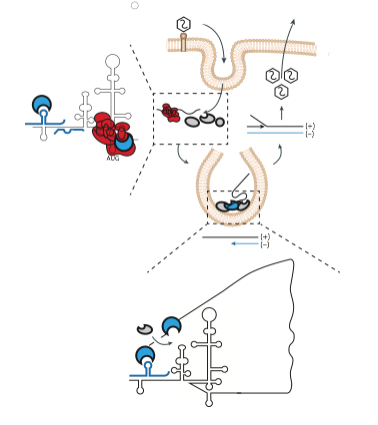
\includegraphics[width=100mm,scale=0.5]{Figures/Fig22}
\caption{Models for PCBP and HCV infection.}
\label{fig:Fig22}
\end{figure*}

In the context of a poliovirus infection, PCBP2 mediates cross-talk between the viral 5$'$ and 3$'$ UTRs in order to regulate the switch between viral translation and RNA replication. Our data are consistent with a symmetrical role for PCBP2 in the context of HCV infection and overlays in vivo biophysical detail from prior reports showing PCBP2-mediates circularization of the HCV genome \emph{in vitro}  \cite{Flynn:2014bi}. Thus, our application of FAST-iCLIP reveals a common binding topology of PCBP2 across the human transcriptome as well as the HCV genome. In both cases, a 3$'$ UTR bias is evident and suggests that PCBP2 regulatory functions may be co-opted by HCV.

\section{Retroviruses}

We have shown, for the first time, that CLIP-seq can be applied to pathogenic RNA viruses. The methods can reveal the molecular interactions between host proteins and the viral genome and is complimentary with high-throughput protein-protein interaction assays that have been applied in similar contexts \cite{Jager:2011de}. Because these interactions are often required for viral replication and translation, information about binding topology can provide insight into mechanism \cite{Walsh:2011kt} as well as reveal new host-viral interactions that guide development of new therapeutic strategies  \cite{Jopling:2005ij}.

We next considered an alternative framing for viral CLIP experiments: the prior work assayed the binding topology of host protein on a viral genome. Could it be possible to investigate the binding of viral protein on host genes (Figure ~\ref{fig:Fig23})?
 
\begin{figure*}
\center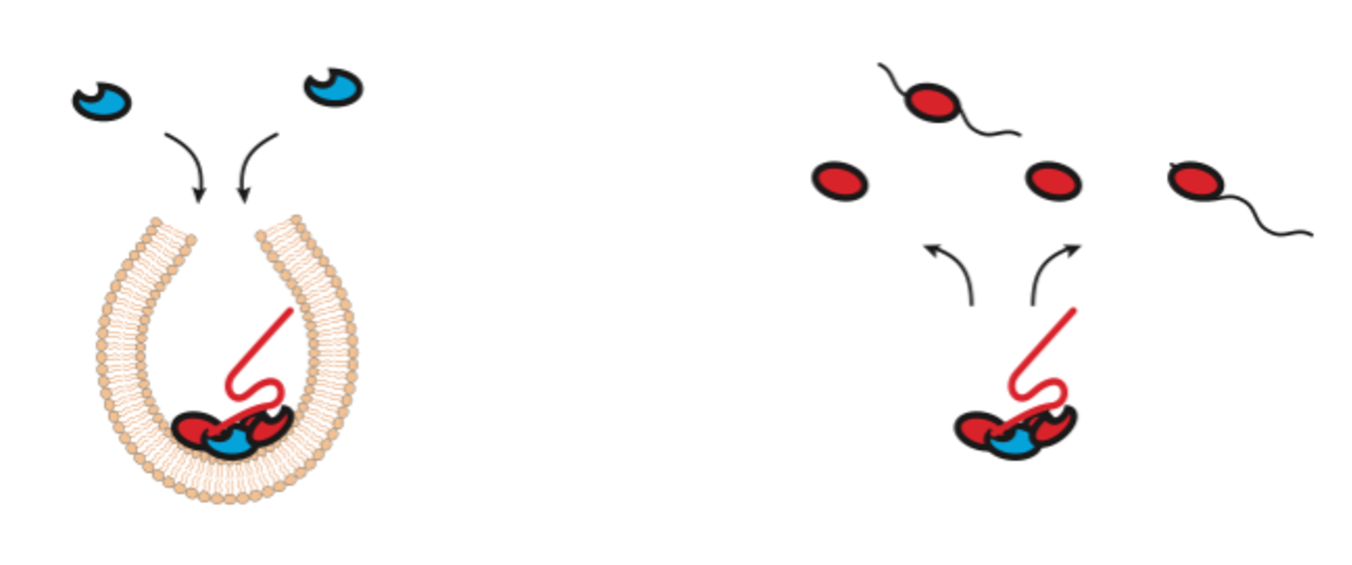
\includegraphics[width=100mm,scale=0.5]{Figures/Fig23}
\caption{CLIP applied to viral proteins.}
\label{fig:Fig23}
\end{figure*}

Addressing this question requires a context in which viral proteins are expected to bind host mRNAs. For this, we turned to retroviruses, RNA viruses characterized by two unique, virally encoded enzymes (reverse transcriptase and integrase) in their lifecycle. These enzymes permit the conversion of RNA into DNA, followed by the integration of viral DNA into the host genome, forming a DNA provirus \cite{Stoye:2012gqa}. Because retroviruses do not usually lyse their target cell, integration allows a long-term association between cell and virus. Numerous studies indicate that such events have occurred multiple times during the course of evolution. Such inherited proviruses are called endogenous retroviruses (ERVs) and they provide a fossil record of past retroviral infections dating back many millions of years. 

Analyses of completed genome sequences have revealed that between four and ten per cent of vertebrate DNA is made up of retroviral remnants \cite{Stoye:2012gqa}. In general, the integrated 5 - 10 kb of sequence encodes for canonical retroviral gag, pol and env genes is flanked by two 300 - 1200 nucleotides bp terminal repeats (LTRs).

Each of these LTRs contains a promoter for RNA polymerase II and enhancers that are responsive to diverse conditions and signals. LTRs are bound by transcription factors, such as enable spatiotemporal control of proviral expression, though many ERV insertions are transcriptionally silenced in embryonic and adult tissues with repressive epigenetic marks \cite{Stoye:2012gqa}. Failure to maintain or contain these silencing marks would result in the reactivation of dormant ERV insertions. In contrast, some ERV-derived sequences that have been incorporated into the normal regulation of mammalian genes (promoters, enhancers or polyadenylation signals). 

\begin{figure*}
\center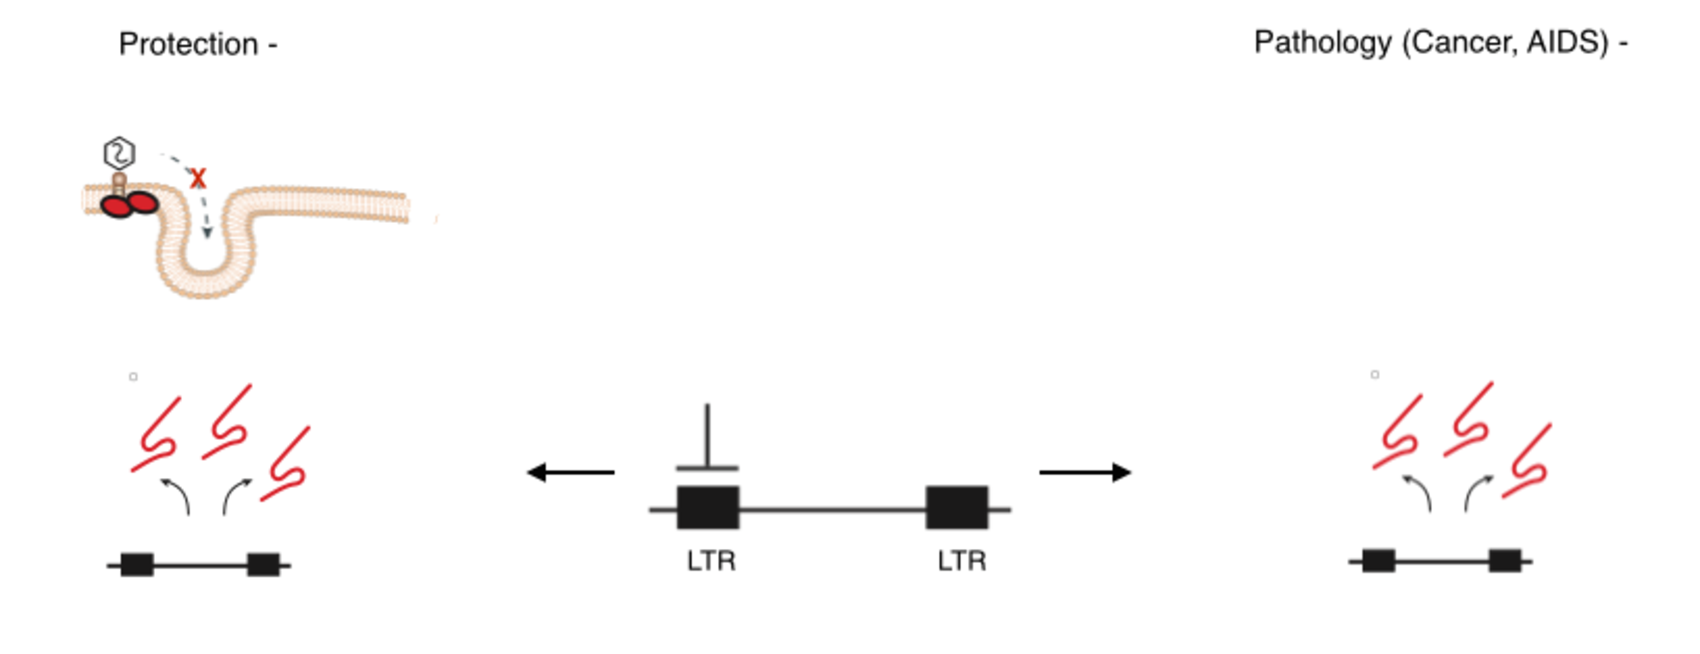
\includegraphics[width=130mm,scale=0.5]{Figures/Fig24}
\caption{Two functional regimes for retroviruses.}
\label{fig:Fig24}
\end{figure*}

ERVs can be therefore thought of as either neutral, beneficial, or harmful. In the harmful case, retrovirses can be re-activated during immunosuppressive disorders, such as AIDS or cancers. Expression of some retroviral Env proteins can modulate the host immune response. These ERV-encoded Env proteins possess immunosuppressive activities that can promote tumorigenesis, as indicated by several studies with mouse cancer models. In contrast, expression of ERV-encoded products can be beneficial. The Jaagsiekte sheep retrovirus (enJSRV) binds cellular receptors, blocking their ability to bind exogenous viral particles \cite{Spencer:2003hv} (Figure ~\ref{fig:Fig24}).

Because retroviral proteins can interact with host factors, we examined the Human ERV-K (HERV-K) subfamily, which is apparently the most recent ERV wave to have entered our genome, perhaps producing insertions as recently as 150,000 years ago. HERV-K retained multiple copies of intact open reading frames (ORFs) that are silenced by the host with exception of certain pathological contexts, such as cancer or HIV \cite{WangJohanning:2003es}. For all human-specific and human-polymorphic HERV-K elements, silencing is mediated by by a specific LTR subgroup, LTR5HS. 

\begin{figure*}
\center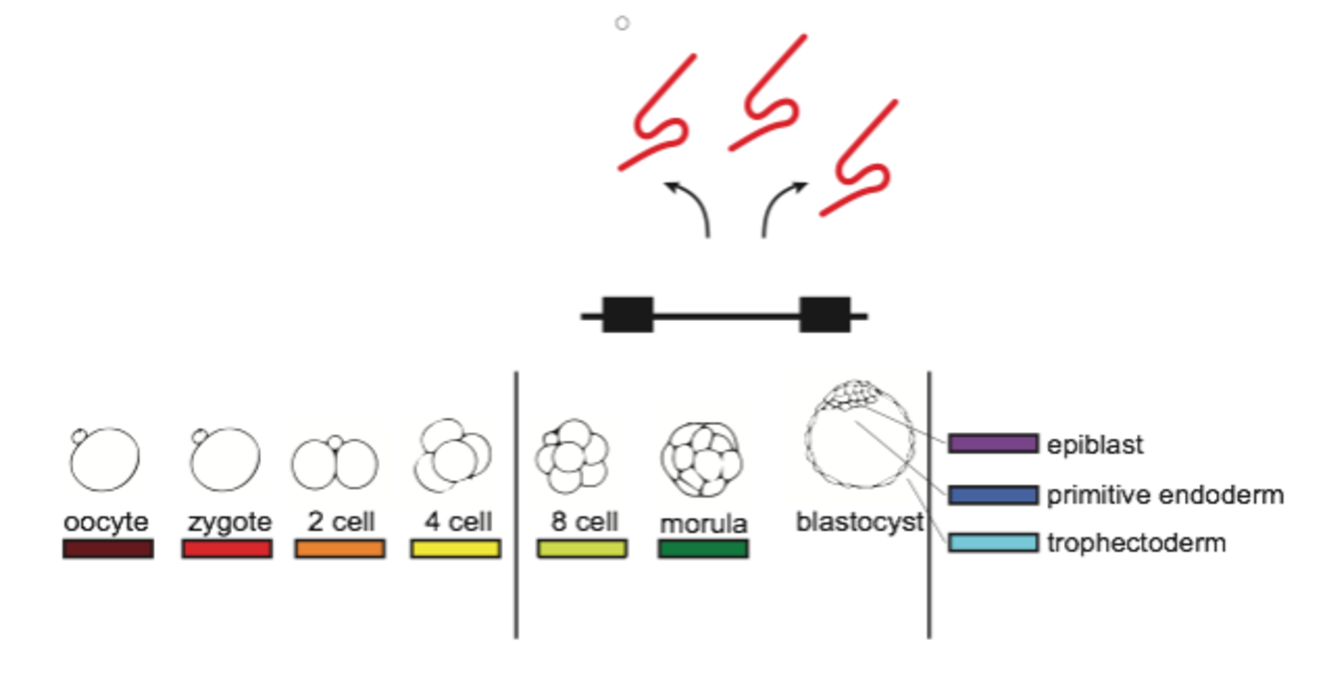
\includegraphics[width=130mm,scale=0.5]{Figures/Fig25}
\caption{HERV-K is expressed in the naive human embryo.}
\label{fig:Fig25}
\end{figure*}

Beyond obvious pathological contexts, recent single-cell RNA-seq has made it possible to examine HERV-K expression in naive embryos prior to blastocyst outgrowth. Analysis of repeat RNAs from single-cell RNA-seq dataset indicates that HERV-K is transcribed at the onset of embryonic genome activation (EGA), at the 8-cell stage, and detected in the embryo prior to EGA \cite{Yan:2013dv}. Human endogenous retrovirus HERV-K and its regulatory element, LTR5HS, were induced after EGA in the 8-cell stage embryos and silenced during blastocyst outgrowth (Figure ~\ref{fig:Fig25}).

Prior studies suggest that retroviral products may be beneficial to the host by preventing exogenous viral infection \cite{WangJohanning:2003es}. We evaluated this by (1) asking whether retroviral products are made in the embyo, (2) examining the interaction between these products at the viral genome for evidence of bona-fide viral activation, and (3) assaying whether retroviral products can influence expression of anti-viral genes.

To evaluate whether HERV-K is functional in embryos, we assayed for the production of viral-like particles (VLPs), which can package viral RNA. We found that HERV-K VLPs indeed assemble in human blastocysts. We then used the CLIP pipeline to assay the viral protein Rec, which promotes nuclear export of viral RNAs. 

\begin{figure*}
\center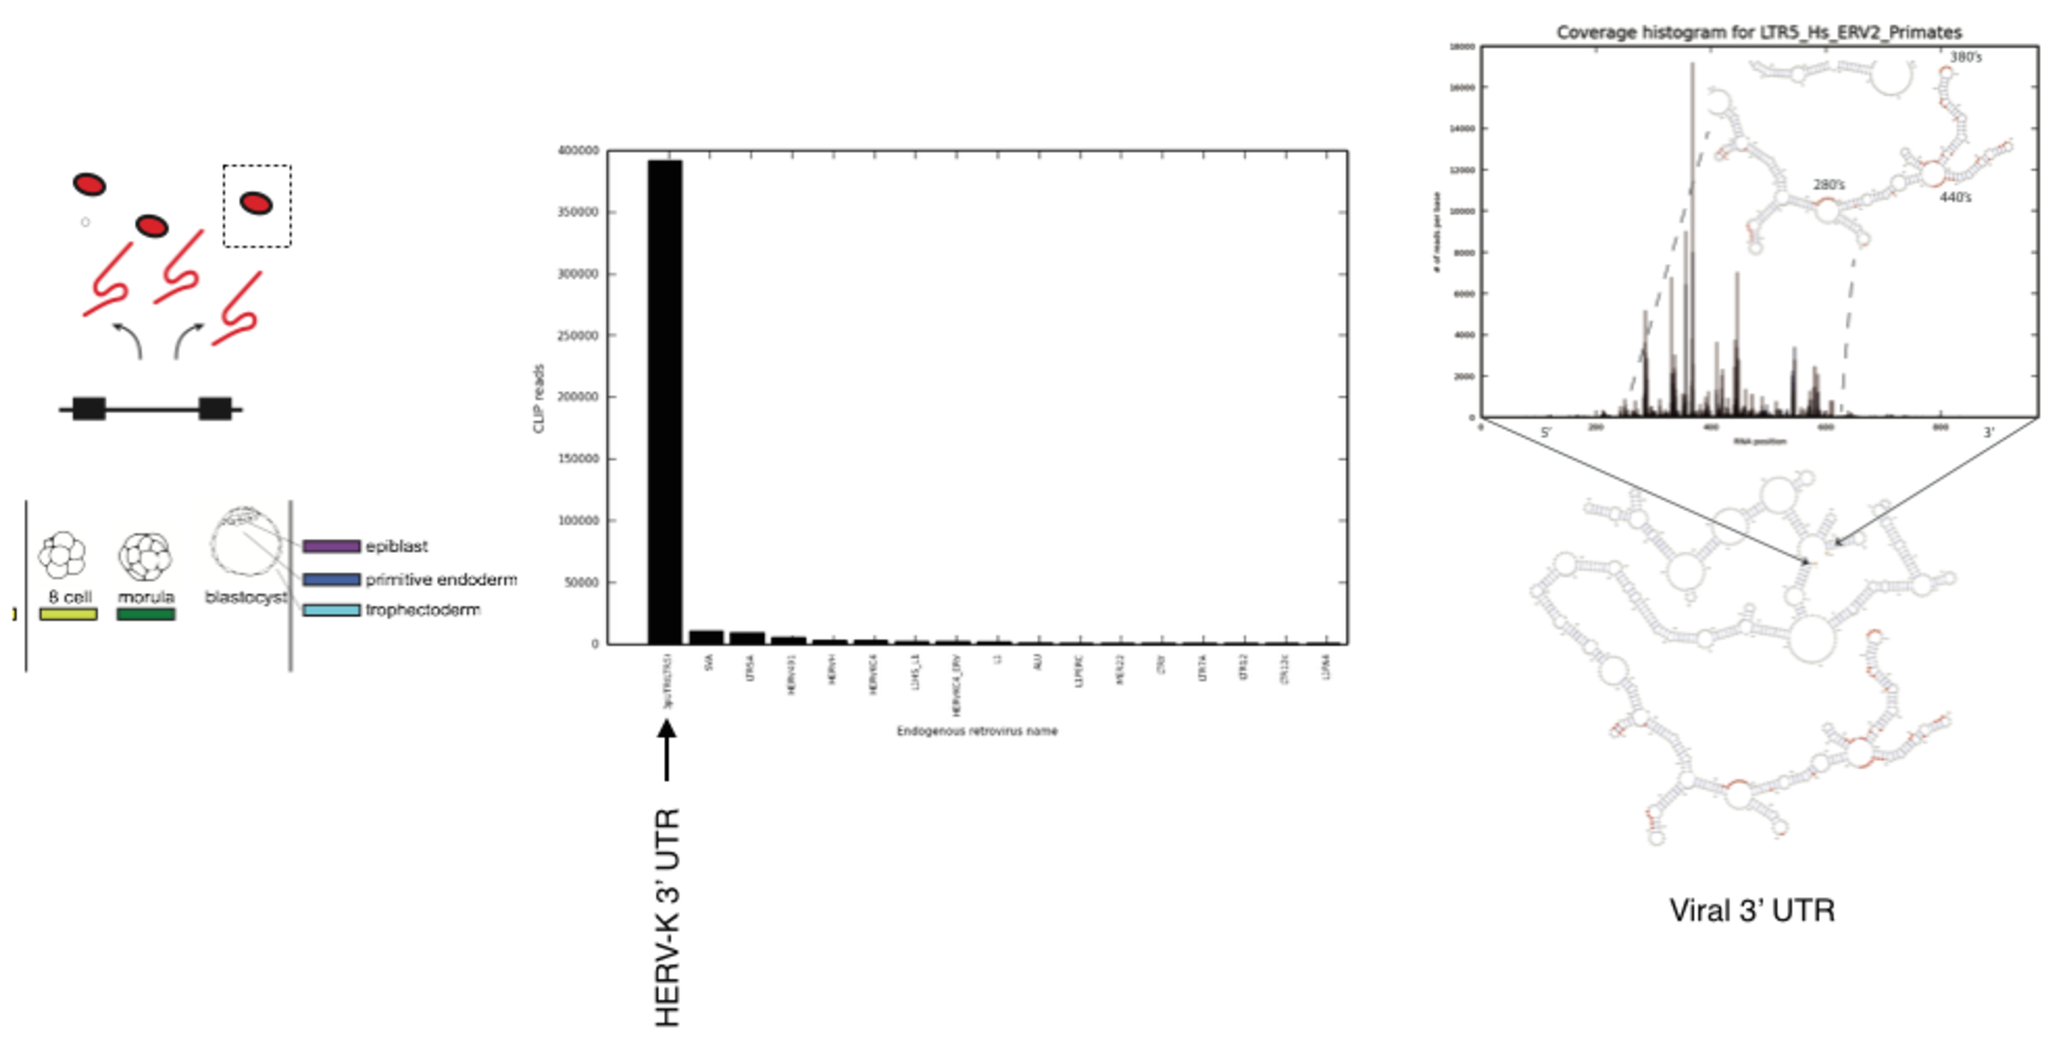
\includegraphics[width=130mm,scale=0.5]{Figures/Fig26}
\caption{Rec binds the 3$'$ UTR of HERV-K in the naive human embryo.}
\label{fig:Fig26}
\end{figure*}

Specifically, Rec is responsible for the export of unspliced and incompletely spliced viral RNAs to the cytosol. Rec binds as an oligomer to a responsive element (RcRE), which is located in the U3 region of the 3$'$ untranslated region of HERV-K transcripts \cite{Lower:tg}. If HERV-K is functional in human embryos, we expect this interaction to be observed. With this in mind, we performed CLIP in human embryonic carcinoma cells (hECCs) for Rec and evaluated the reads using a custom retroviral genome index that contained HERV-K as well as its UTR elements. We observed a strong signal in 3' UTR of the virus (Figure ~\ref{fig:Fig25}) in the region expected, the RcRE, which is indicative of viral activation in the embryo. 

With this in mind, we asked whether Rec-mediated nuclear export of viral RNAs into the cytoplasm might lead to the upregulation of innate anti-viral response genes. We observed a striking upregulation of a viral restriction factor IFITM, with around 700 fold induction in human blastocysts as compared to pre-EGA (4-cell and 8-cell stage) embryos. IFTIM1, an interferon induced transmembrane protein, is thought to protect cells from viral infection at an early step by blocking endocytosis of virions into the cytosol. We also found that Rec overexpression is sufficient to increase IFITM1 levels in hECCs, the cell line in which we performed the CLIP. 

\begin{figure*}
\center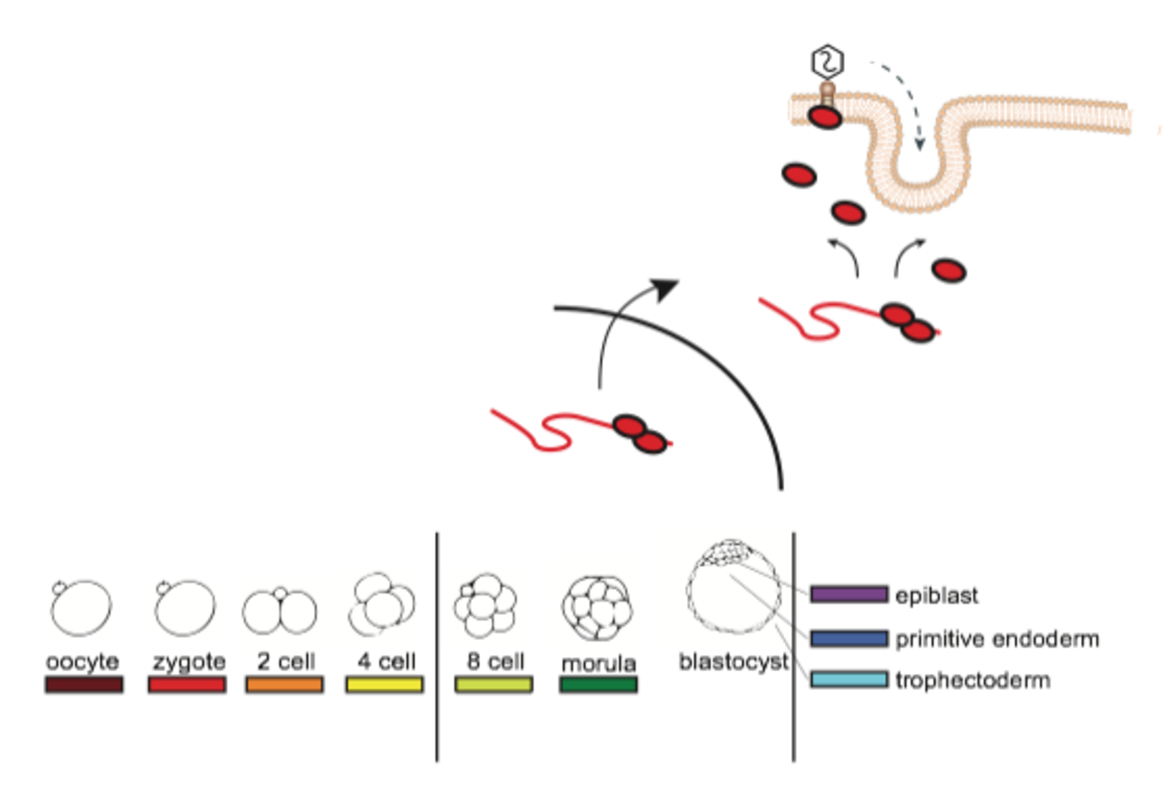
\includegraphics[width=100mm,scale=0.5]{Figures/Fig27}
\caption{Retrovirals products in human embryo.}
\label{fig:Fig27}
\end{figure*}

Collectively, these results indicate that pre-implantation development proceeds in the presence of retroviral proteins, which may induce viral restriction factors that protect the embryo from exogenous infection. We used CLIP to evaluate the interaction network of a protein, Rec, that is critical in the HERV-K lifecycle. These results provide further evidence for activation of HERV-K and also reveal a cryptic network of interactions between Rec and host RNAs, which must be further characterized. 
